% $Id: template.tex 11 2007-04-03 22:25:53Z jpeltier $

\documentclass{vgtc}                          % final (conference style)
%\documentclass[review]{vgtc}                 % review
%\documentclass[widereview]{vgtc}             % wide-spaced review
%\documentclass[preprint]{vgtc}               % preprint
%\documentclass[electronic]{vgtc}             % electronic version

%% Uncomment one of the lines above depending on where your paper is
%% in the conference process. ``review'' and ``widereview'' are for review
%% submission, ``preprint'' is for pre-publication, and the final version
%% doesn't use a specific qualifier. Further, ``electronic'' includes
%% hyperreferences for more convenient online viewing.

%% Please use one of the ``review'' options in combination with the
%% assigned online id (see below) ONLY if your paper uses a double blind
%% review process. Some conferences, like IEEE Vis and InfoVis, have NOT
%% in the past.

%% Figures should be in CMYK or Grey scale format, otherwise, colour 
%% shifting may occur during the printing process.

%% These few lines make a distinction between latex and pdflatex calls and they
%% bring in essential packages for graphics and font handling.
%% Note that due to the \DeclareGraphicsExtensions{} call it is no longer necessary
%% to provide the the path and extension of a graphics file:
%% 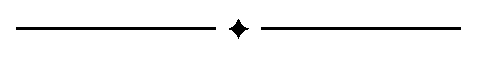
\includegraphics{diamondrule} is completely sufficient.
%%
\ifpdf%                                % if we use pdflatex
  \pdfoutput=1\relax                   % create PDFs from pdfLaTeX
  \pdfcompresslevel=9                  % PDF Compression
  \pdfoptionpdfminorversion=7          % create PDF 1.7
  \ExecuteOptions{pdftex}
  \usepackage{graphicx}                % allow us to embed graphics files
  \DeclareGraphicsExtensions{.pdf,.png,.jpg,.jpeg} % for pdflatex we expect .pdf, .png, or .jpg files
\else%                                 % else we use pure latex
  \ExecuteOptions{dvips}
  \usepackage{graphicx}                % allow us to embed graphics files
  \DeclareGraphicsExtensions{.eps}     % for pure latex we expect eps files
\fi%

%% it is recomended to use ``\autoref{sec:bla}'' instead of ``Fig.~\ref{sec:bla}''
\graphicspath{{figures/}{pictures/}{images/}{./}} % where to search for the images

\usepackage{microtype}                 % use micro-typography (slightly more compact, better to read)
\PassOptionsToPackage{warn}{textcomp}  % to address font issues with \textrightarrow
\usepackage{textcomp}                  % use better special symbols
\usepackage{mathptmx}                  % use matching math font
\usepackage{times}                     % we use Times as the main font
\renewcommand*\ttdefault{txtt}         % a nicer typewriter font
\usepackage{cite}                      % needed to automatically sort the references
\usepackage{tabu}                      % only used for the table example
\usepackage{booktabs}                  % only used for the table example
%% We encourage the use of mathptmx for consistent usage of times font
%% throughout the proceedings. However, if you encounter conflicts
%% with other math-related packages, you may want to disable it.


%% If you are submitting a paper to a conference for review with a double
%% blind reviewing process, please replace the value ``0'' below with your
%% OnlineID. Otherwise, you may safely leave it at ``0''.
\onlineid{0}

%% declare the category of your paper, only shown in review mode
\vgtccategory{Research}

%% allow for this line if you want the electronic option to work properly
\vgtcinsertpkg

%% In preprint mode you may define your own headline. If not, the default IEEE copyright message will appear in preprint mode.
%\preprinttext{To appear in an IEEE VGTC sponsored conference.}

%% This adds a link to the version of the paper on IEEEXplore
%% Uncomment this line when you produce a preprint version of the article 
%% after the article receives a DOI for the paper from IEEE
%\ieeedoi{xx.xxxx/TVCG.201x.xxxxxxx}


%% Paper title.

\title{Event HyperGraph for analyzing large collections of text}

%% This is how authors are specified in the conference style

%% Author and Affiliation (single author).
%%\author{Roy G. Biv\thanks{e-mail: roy.g.biv@aol.com}}
%%\affiliation{\scriptsize Allied Widgets Research}

%% Author and Affiliation (multiple authors with single affiliations).
%%\author{Roy G. Biv\thanks{e-mail: roy.g.biv@aol.com} %
%%\and Ed Grimley\thanks{e-mail:ed.grimley@aol.com} %
%%\and Martha Stewart\thanks{e-mail:martha.stewart@marthastewart.com}}
%%\affiliation{\scriptsize Martha Stewart Enterprises \\ Microsoft Research}

%% Author and Affiliation (multiple authors with multiple affiliations)
\author{Sam Yu-Te Lee\thanks{e-mail: ytlee@ucdavis.edu}\\ %
        \scriptsize University of California, Davis %
\and Kwan-Liu Ma\thanks{e-mail: klma@ucdavis.edu}\\ %
     \scriptsize University of California, Davis %
}

%% A teaser figure can be included as follows
% \teaser{
%   \centering
%   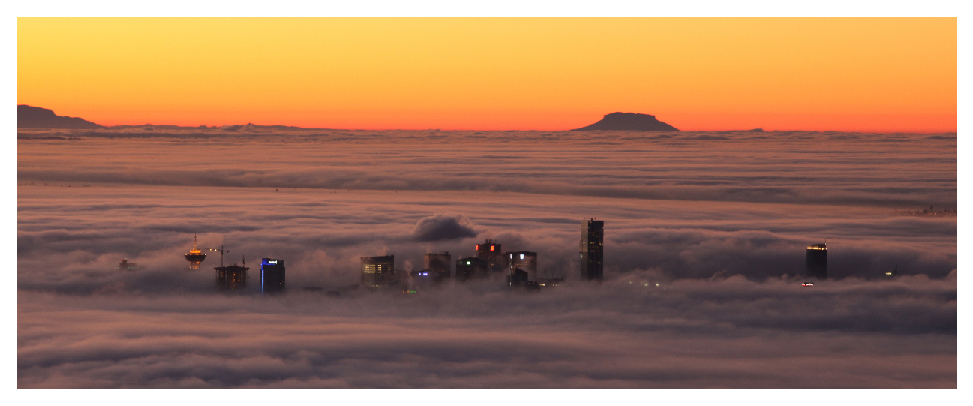
\includegraphics[width=\linewidth]{CypressView}
%   \caption{In the Clouds: Vancouver from Cypress Mountain. Note that the teaser may not be wider than the abstract block.}
%   \label{fig:teaser}
% }

%% Abstract section.
\abstract{Duis autem vel eum iriure dolor in hendrerit in vulputate
velit esse molestie consequat, vel illum dolore eu feugiat nulla
facilisis at vero eros et accumsan et iusto odio dignissim qui blandit
praesent luptatum zzril delenit augue duis dolore te feugait nulla
facilisi. Lorem ipsum dolor sit amet, consectetuer adipiscing elit,
sed diam nonummy nibh euismod tincidunt ut laoreet dolore magna
aliquam erat volutpat. Ut wisi enim ad minim veniam, quis nostrud exerci tation ullamcorper
suscipit lobortis nisl ut aliquip ex ea commodo consequat. Duis autem
vel eum iriure dolor in hendrerit in vulputate velit esse molestie
consequat, vel illum dolore eu feugiat nulla facilisis at vero eros et
accumsan et iusto odio dignissim qui blandit praesent luptatum zzril
delenit augue duis dolore te feugait nulla facilisi.%
} % end of abstract

%% ACM Computing Classification System (CCS). 
%% See <http://www.acm.org/about/class> for details.
%% We recommend the 2012 system <http://www.acm.org/about/class/class/2012>
%% For the 2012 system use the ``\CCScatTwelve'' which command takes four arguments.
%% The 1998 system <http://www.acm.org/about/class/class/2012> is still possible
%% For the 1998 system use the ``\CCScat'' which command takes four arguments.
%% In both cases the last two arguments (1998) or last three (2012) can be empty.

\CCScatlist{
  \CCScatTwelve{Human-centered computing}{Visu\-al\-iza\-tion}{Visu\-al\-iza\-tion techniques}{Treemaps};
  \CCScatTwelve{Human-centered computing}{Visu\-al\-iza\-tion}{Visualization design and evaluation methods}{}
}

%\CCScatlist{
  %\CCScat{H.5.2}{User Interfaces}{User Interfaces}{Graphical user interfaces (GUI)}{};
  %\CCScat{H.5.m}{Information Interfaces and Presentation}{Miscellaneous}{}{}
%}

%% Copyright space is enabled by default as required by guidelines.
%% It is disabled by the 'review' option or via the following command:
% \nocopyrightspace

%%%%%%%%%%%%%%%%%%%%%%%%%%%%%%%%%%%%%%%%%%%%%%%%%%%%%%%%%%%%%%%%
%%%%%%%%%%%%%%%%%%%%%% START OF THE PAPER %%%%%%%%%%%%%%%%%%%%%%
%%%%%%%%%%%%%%%%%%%%%%%%%%%%%%%%%%%%%%%%%%%%%%%%%%%%%%%%%%%%%%%%%

\begin{document}

%% The ``\maketitle'' command must be the first command after the
%% ``\begin{document}'' command. It prepares and prints the title block.

%% the only exception to this rule is the \firstsection command
% \firstsection{Introduction}

\maketitle
\section{Introduction}
Text data is ubiquitous.
From news articles and social media posts to scientific publications, the tremendous amount of text data that is produced poses not only opportunities but also a great challenge to anyone who needs to analyze them.
Visual analytics (VA) mitigates this challenge by combining mathematical models and visualizations to automate the sensemaking process and reduce the cognitive load.
Chuang et al.~\cite{chuang2012interpretation} proposed that \textit{Model alignment}, the alignment of analysis tasks, visual encodings and model decisions,
greatly affects users' interpretation and trust in visual analytic systems.
However, in text analysis, the available models often align poorly with analysis tasks.
For example, topic models are commonly used to model the topical structure of text documents.
Most topic models characterize \textit{topic} as a probabilistic distribution spanning a given vocabulary~\cite{vayansky2020review}.
This transformation from \textit{topics}, a high-level concept that the user seeks to understand, to a \textit{probabilistic distribution}, a low-level concept that mathematical models can operate on, prevents proper model alignment.
The misalignment between analysis tasks and models limits the usage of visual analytics systems for users who are not familiar with the underlying models.

Recent advances in large language models (LLM) present a promising solution to this problem.
LLMs have proven successful in various natural language processing (NLP) tasks, especially in question-answering tasks due to their strong capability to understand user intent.
Researchers in visualization have adopted LLMs to assist data transformation~\cite{wang2023dataformulator} or directly generate visualization~\cite{maddigan2023chat2vis}.
However, they all assumed a clean data format, where the data to be visualized is already in a table format. 
For unstructured text analysis though, this is rarely the case.
Topics~\cite{atzberger2023evaluatetopicmodel}, sentiments~\cite{beasley2021through}, concepts and entities~\cite{park2018conceptvector,cao2010facetatlas} are common analysis targets in text analysis, which require a data preparation stage to extract them from unstructured text.
Recently, Li et al.~\cite{li2023evaluateChatgpt} evaluated ChatGPT's capabilities on Information Extraction (IE) tasks comprehensively, and found that it excels under an OpenIE setting, where the model relies solely on user input to extract information from documents.
The capability of LLMs to extract information from documents according to user intent eliminates the need to carefully align the analysis tasks and models in VA systems,
because a specific model is no longer needed to prepare the data for the analysis task.
In the previous example, instead of relying on abstruse and unfathomable probabilistic models, LLMs can directly process the text data and summarize the topics of the documents.
A user can ask a LLM:\@ \textit{`What are the topics of these articles?'}, and the LLM would give a human-like response, such as \textit{`The articles are about \ldots'}.

However, using LLMs in the data preparation stage is not trivial. 
Problems like \textit{hallucination} and \textit{faithfulness} hinder the accuracy of the extracted information.
Token limits restrict the length of the input text, limiting the usage of LLMs on large collections of documents (corpus).
Prompts need to be carefully designed to reflect user intent.
Finally, the extracted information, the analysis task and the visualization need to be aligned to foster interpretation and trust.
In this work, we designed a VA system that models a corpus as a hypergraph, where the nodes are articles and salient entities (or concepts) extracted from the articles.
We showcase how LLMs are used flexibly to align the data, analysis task and visualization during our design process.
The hypergraph is then hierarchically clustered and visualized by extending space-filling curve layouts~\cite{muelder2008sfc}.
The system supports interactive exploration, reorganization and analysis of the documents.
To the best of our knowledge, no visual analytics system has adopted LLMs to assist the data preparation stage in text analysis.
Using the system, we demonstrate how proper model alignment can be achieved using LLMs.

The contributions of our work are as follows:
\begin{itemize}
    \item We introduce an LLM-based information extraction pipeline that is capable of extracting topics and salient entities from a given corpus in a way that fosters interpretation.
    \item We extend space-filling curve layouts to visualize clusters in large hypergraphs.
    \item We develop a novel VA system that allows users to effectively explore, reorganize and analyze a corpus.
\end{itemize}











\section{Related Works}
\section{Design Rationale}~\label{sec: design_rationale}
What DRs are needed for analysts to explore and reorganize a corpus for their analytical tasks and why?
\subsection{Design Considerations}
\begin{itemize}
    \setlength\itemsep{0em}
      \item \textbf{DC1: An overview of the topic structure} 
      \item \textbf{DC2: Support for curation through user interaction } 
      \item \textbf{DC3: Detailed analysis of the curated result } 
  \end{itemize}
\section{Methodology}\label{sec: methodology}
As shown in~\autoref{fig:pipeline}, starting from a corpus of unstructured texts,
we first use LLMs to extract the main characters from each document.
The characters are disambiguated and linked to a knowledge base if available.
We create and store the document embeddings and character embeddings for further usage.
All LLM-based preprocessing used OpenAI's\footnote{\url{https://platform.openai.com}} `gpt-3.5-turbo-16k-0613' model.
We provide all our prompts in supplemental material.
In the next stage, we construct a document hypergraph and a character hypergraph, which are then clustered separately by combining connectivity similarity and semantic similarity.
The clustering result is hosted on the server and visualized in an interactive user interface.
Below, we describe each component in detail.
\subsection{Data Preparation}\label{sec: preprocessing}
\subsubsection{Datasets}
The scope of this research paper is to visualize unstructured data conveying any type of information. 
We evaluate our system on two different datasets: the \textit{All The News} dataset~\cite{allthenews} and a visualization publication dataset (VisPub)~\cite{vispub}.
\begin{itemize}
    % \item Roles Across Multiple Sentences (RAMS) - This dataset contains news articles with a wide variety of events. It contains 9,124 annotated events with 135 event types and 65 roles. We have used this dataset because of its abstract and wide ranging information that is not just restricted to a specific domain. 
    \item \textbf{All The News} \, This dataset contains 2.7 million articles from 27 American publications.  It typically includes metadata such as headlines, publication dates, and the full text of the articles. For our purpose, we only use the full text of the articles in our pipeline. We down-sampled the dataset to contain only 10 percent of articles published in 2016. This resulted in a dataset of 8192 articles. We used this subset to evaluate our system in a case study.
    \item \textbf{Visualization Publications Dataset (VisPub)} \, This dataset contains 3620 IEEE visualization publications from 1990 to 2022. We removed 79 articles that do not have abstracts available. These research papers cover a wide variety of research topics in visualization, which is not necessarily known to LLMs. We tested our system on this dataset to show that our system does not rely on the parametric knowledge learned by LLMs during training.
\end{itemize}
\subsubsection{Summarization}\label{sec: summarization}
Unstructured text documents can contain a vast amount of information, among which certain information is more important than others.
Summarization helps condense the content into a concise form, making it easier for users to make sense of and LLMs to process and extract the most important information. 
Zhang et al\cite{zhang2023extractive} reported that human users found the summaries generated by ChatGPT to be more interpretable and trustworthy than traditional approaches, which makes LLMs a better choice for our purpose.
For the VisPub dataset, the abstracts of research papers already convey the main research idea in a condensed form, therefore the abstracts were used as a summary of the document.
We employed an instruction-based zero-shot prompt, where the model is instructed to act as a text summarizer given the document's content, as shown in the following: 
\textit{`You are a summarization system that summarizes the events that happened between the main characters of a news article.
The user will provide you with a news article to summarize.
Try to summarize the article with no more than three sentences. 
Reply starts with 'The article discussed ...''}.
Although we instructed the model to generate a summary with no more than three sentences, we found that the model often does not adhere to that instruction.
It is simply a signal to the model that the summary should be concise.
These summaries are used in subsequent preprocessing stages as well as in the user interface.

\subsubsection{Character Extraction}\label{sec: character_extraction}
The character extraction builds upon the summaries generated in the previous step.
We define a character as entities or concepts that are significantly discussed in the documents.
For news articles, a character can be a person, place or location.
For research papers, a character can be a model, a technique or an algorithm proposed or used by the paper.
Previous works use computational metrics such as TF-IDF or \textit{saliency} to extract characters.
However, computational metrics often cannot well encode high-level semantics.
Instead, we rely on LLMs' ability to understand natural language to identify significant characters from unstructured texts.

We broke down the process of character extraction into two steps to avoid the problem of extrinsic hallucination as discussed by Bang et al.~\cite{bang2023multitask}.
First, a sentence describing the most important event is generated from the summary. 
The event should be the primary focus of the news article and should describe the major objective of the news article, such as a geopolitical event like the G20 summit.
An instruction-based prompt with a few-shot learning approach was adopted to give the LLM an example of what kind of events would be described as the main event. 
Next, all the main characters involved in that event are extracted with an opinion-based few-shot prompt.
The prompt transforms an extraction task into an opinion-seeking task.
An example prompt used in the \textit{All The News} dataset is 
`A major event is reported by a news article: \{event\},
what are the main characters that are majorly involved in the event?'.
This step yields better results if the model already knows what event is happening.
Also, since the event is given as context for this step, the chances of generating a hallucinated output are reduced.
The extracted characters will then be disambiguated and used to construct the hypergraph.

\subsubsection{Character Disambiguation}\label{sec: character_disambiguation}
Once the main characters are extracted, a disambiguation step is done to create connections between documents.
In early experiments, we found that LLMs do not excel at disambiguating characters.
We thus prioritize using an entity linking model to disambiguate characters.
Entity linking is the task of mapping a named entity text mentions to their corresponding entities in a knowledge base~\cite{shen2014entity}.
Existing models adopt a supervised learning approach, where a large amount of training data is required, so they are usually limited to a specific domain.
For datasets that an existing entity-linking model is available, we use it to disambiguate characters.
For example, to process the \textit{All The News} dataset, we used ReFinED~\cite{ayoola2022refined}, an entity linking model that maps text mentions to entities in Wikipedia or Wikidata.
In cases where the characters cannot be linked to an external knowledge base, like the \textit{VisPub} dataset, we employ a matching algorithm based on embeddings.
The algorithm is straightforward:
For every main character extracted in the previous step, we embed them and create a pair-wise similarity matrix.
Then the pairs of characters with a similarity score above a threshold are considered to be the same character.
We then use LLMs to generate a unified title for the matched characters, which is used as the character's label in the user interface.

\subsubsection{Document and Character Embedding}\label{sec: embeddings} 
Embeddings are dense vectors that can be used to measure similarities between objects.
In text analysis, embeddings are often created on words, sentences or documents.
We adopted a similar approach here for both documents and characters.
For documents, we embed the summaries generated in~\autoref{sec: summarization}.
For characters that can be linked to an external knowledge base,
we embed the description section of the character in the knowledge base.
Otherwise, we embed all text mentions that appear in the corpus and average them to generate the embedding for a disambiguated character.
We used OpenAI's `text-embedding-ada-002' model for all embeddings. 
This allows us to measure the semantic similarity between documents, characters and user queries in the same vector space.

\subsubsection{Topic Label Generation}\label{sec: tag_assignment}
Later in the preprocessing pipeline, we will use a hierarchical clustering algorithm to cluster the documents and characters (described in~\autoref{sec: clustering}). 
The algorithm outputs a hierarchy, where leaf nodes are documents or characters and internal nodes are clusters.
The clustering result faces a similar problem with embedding-based approaches, where the clusters are not interpretable.
To address this issue, we use LLMs to assign human-like labels to each cluster.
Our approach is similar to a recent work done by Raval et al.~\cite{raval2023explainandtrust}, where they use LLMs to generate explanations for a user-selected set of points.
However, our task is more complicated because the prompt needs to (1) consider the hierarchical information, and (2) be able to process large clusters containing thousands of documents without breaking the token limit.

We describe our topic label generation process in a bottom-up manner:
(1) At the bottom level (one level above the leaf nodes), assign topic labels to the clusters using the document summaries;
(2) At any level above, assign labels to the clusters using the labels of their children and randomly sampled document summaries.

The first step is straightforward, where we simply use the document to generate labels for each cluster.
The bottom-level clusters usually contain only a few documents, so the token limit is unlikely to be exceeded.
We insert the summarization generated in~\autoref{sec: summarization} into the prompt template.
The prompt instructs the LLM to generate a label composed of a single noun phrase for the given documents.

Then at any level above, the cluster size increases dramatically and the token limit is likely to be exceeded.
To solve this problem, we first insert the labels of a cluster's children instead of the document.
This guarantees that the token limit will not be exceeded.
In early experiments, we found that the children's labels alone were not enough to generate a meaningful label for the parent cluster.
Therefore, we also insert documents randomly sampled from the cluster.
We enforce that each child has at least one article being sampled, and distribute the remaining token space proportionally to the size of each child.

\subsection{Models}
\subsubsection{Hypergraph Construction}
A hypergraph is a generalization of a graph in which an edge can connect any number of nodes~\cite{fischer2021hypergraphsurvey}.
A hyperedge thus represents a multi-way relationship between nodes.
In our work, we model two types of hypergraphs: document hypergraph and character hypergraph.
In a document hypergraph, the nodes are documents and the hyperedges are characters.
Similarly, in a character hypergraph, the nodes are characters and the hyperedges are documents.
Analyzing the document hypergraph and character hypergraph correspond to topic-based and entity-based analysis, respectively.
By modeling the corpus as hypergraphs, the system supports users to conduct both types of analysis simultaneously under a unified framework (\textbf{DC1}).
Below, we explain the relation between these two types of hypergraphs and how they are constructed.

Following the definition of a hypergraph node, a hyperedge can be used to represent two types of multi-way relationships:
In a document hypergraph, a hyperedge (connecting document nodes) can be constructed between documents that mention the same character. 
In this case, the hyperedge represents the co-mention of a character.
In a character hypergraph, a hyperedge (connecting character nodes) can be constructed between characters if they are mentioned together in the same document.
In this case, the hyperedge represents a co-occurrence relationship between characters.
This means the two hypergraphs are both built from the same corpus, using the same relationship information, but from different perspectives.
Once the two hypergraphs are constructed, we further separately cluster them hierarchically.
Clusters in the document hypergraph represent topics that are discussed in the dataset.
Clusters in the character hypergraph represent characters (entities or concepts) that are similar to each other.
For better interpretability of the clustering result, we further assign \textit{labels} to each cluster, as explained in~\autoref{sec: tag_assignment}.

Although these two types of hypergraphs are constructed from different perspectives, we utilize the \textit{dual} of a hypergraph to simplify the construction process.
The dual of a hypergraph is simply another hypergraph, where the nodes and hyperedges are interchanged, as shown in~\autoref{fig: duality}.
Using the duality feature, we first model the documents as nodes and characters as hyperedges to construct the document hypergraph $H_D$.
The character hypergraph $H_C$ can then be easily constructed by taking the dual of $H_D$.
This construction process also allows us to map user interactions on documents and characters to operations on a single hypergraph (\textbf{DC1}).
Even better, the duality feature between documents and characters matches the user's mental model (\textbf{DC3}), making the visualization and interaction intuitive.

\begin{figure}
 \centering % avoid the use of \begin{center}...\end{center} and use \centering instead (more compact)
 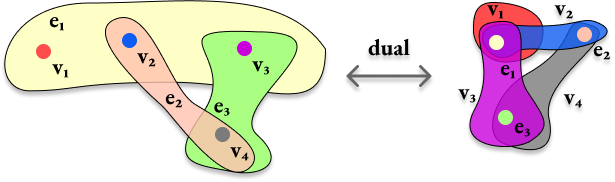
\includegraphics[width=\columnwidth]{duality}
 \captionsetup{belowskip=-14pt,aboveskip=3pt}
 \caption{Illustration of the dual of a hypergraph. 
 Left: a hypergraph with 4 nodes $v_1, v_2, v_3, v_4$ and 3 hyperedges $e_1=(v_1, v_2, v_3), e_2=(v_2, v_3), e_3=(v_3, v_4)$. 
 Right: the dual of the hypergraph, where the nodes and hyperedges interchanged.
 Nodes in the dual hypergraph are now $e_1, e_2, e_3$ and hyperedges are $v_1=(e_1), v_2=(e_1, e_2), v_3=(e_1, e_3), v_4=(e_2, e_3)$.
 }

\label{fig: duality}
\end{figure}

\subsubsection{Hierarchical Clustering}\label{sec: clustering}
Common clustering algorithms for graphs consider only graph connectivity.
However, for the best interpretability of the clustering result, the node embeddings must be also used in the clustering process.
This limits our choice of clustering algorithms to attributed node clustering algorithms.
Although there are existing approaches that can cluster attributed nodes on graphs such as EVA~\cite{citraro2020eva} and iLouvain~\cite{combe2015louvain}, they are not designed for hypergraphs.
In general, hypergraphs can be clustered in two different ways: 
(1) Directly operate on the hyperedges by generalizing the graph clustering algorithms.
For example, Kamiński et al.~\cite{kaminski2021hgraphcommunity} generalizes the modularity metric for graphs to hypergraphs; 
(2) First transform the hypergraph into a graph and then apply normal graph clustering algorithms~\cite{kumar2020new}.
Although the first approach is more intuitive, it is less scalable and hard to incorporate node attributes.
Thus, we have decided to design our clustering algorithm following the second approach.

Considering all the above, we implemented our hierarchical clustering algorithm by first transforming the hypergraph into a graph following the edge re-weighting process proposed by Kumar et al.~\cite{kumar2020new}.
Then an agglomerative clustering algorithm~\cite{steinbach2000doccluster} is applied on the re-weighted graph.
In agglomerative clustering, the key is to define node similarity and cluster similarity.
We can easily incorporate node attributes into the clustering process by defining the similarity between nodes and clusters as a weighted sum of attribute similarity $S_s$ and connectivity similarity $S_c$.
Since we're dealing with texts, we refer to the attribute similarity between nodes as semantic similarity. 

The semantic similarity $S_s(i, j)$ is the cosine similarity of the embeddings (dense vectors) of the two nodes, denoted as $vec_i$ and $vec_j$.
% For article nodes, the embeddings are generated using the article summaries.
% For participant nodes, the embeddings are generated using a description note of the participant.
% More details about the embeddings are explained in~\autoref{sec: embeddings}.
The connectivity similarity $S_c$ is the weighted Topological Overlap (wTO)~\cite{gysi2018wto},
which is a weighted generalization of the Overlap Coefficient~\cite{vijaymeena2016survey}, as shown in~\autoref{eq: connectivity_semantic_similarity}.
\begin{equation}\label{eq: connectivity_semantic_similarity}
    \mathbf{S_s}(i, j) = \frac{vec_i \cdot vec_j}{||vec_i|| \cdot ||vec_j||}, \quad
    \mathbf{S_c}(i, j) = \frac{\sum_{u=1}^N{w_{i,u}w_{u_j}} + w_{i,j}}{\min(k_i, k_j) + 1 - |w_{i,j}|}
\end{equation}
where $k_i = \sum_{j=1}^N |w_{i,j}|$ is the total weight of the edges connected to node $i$.
Finally, a weighting factor $\alpha$ is used to balance the two similarities, as shown in~\autoref{eq: similarity}.
\begin{equation}\label{eq: similarity}
    \mathbf{S} = \alpha \mathbf{S_s} + (1-\alpha) \mathbf{S_c}
\end{equation}
For the similarity between clusters, we used centroid similarity, i.e.\ the similarity between two clusters is the similarity between the centroids of the two clusters.
The algorithm takes a hypergraph $H=(V, E)$ and the embeddings of each node $Vec$ as input, and outputs a sequence of partitions $P=P_1, P_2, \dots P_k$.
Each partition corresponds to a level in the hierarchy, as shown in Algorithm 1.
\begin{algorithm}\label{alg: clustering}
    \caption{Agglomerative Clustering }\label{alg:cap}
    \hspace*{\algorithmicindent} \textbf{Input}: $H=(V, E)$, $Vec=\{vec_i |\, i \in V\}$ \\
    \hspace*{\algorithmicindent} \textbf{Output}: Sequence of partitions $\mathbf{P}=P_1, P_2, \dots P_k$ \\
    \begin{algorithmic}[1]
    \While{$|V| > 1$}
        \State$P_k = init\_partition(V)$ \Comment{Initialize each node as a cluster}
        \State$\mathbf{S_s} = cosine\_similarity(V\times V, Vec)$ 
        \State$\mathbf{S_c} = wTO(V\times V, E)$ \
        \For{$i \in V$}
            \State$j = most\_similar\_node(i, S_s, S_c)$ 
            \State$P_k = merge\_clusters(i, j)$ \Comment{Merge the two clusters}
        \EndFor
        \State$H^\prime=(V^\prime, E^\prime) = construct\_hypergraph(P_k)$ \Comment{clusters are the new nodes}
        \State$Vec^\prime = centroid\_similarity(V^\prime)$
        \State$V=V^\prime, E=E^\prime, Vec=Vec^\prime$ \Comment{Update for next iteration}
    \EndWhile
    \end{algorithmic}
\end{algorithm}



\section{Visualization}~\label{sec: visualization}
\subsection{SFC for HyperGraph}

In the design guidelines proposed by Abdelaal et al.~\cite{abdelaal2022network} in a recent network visualization evaluation study, node-link-based approaches are recommended when:
(1) tasks involve the identification of network clusters, and (2) the network is sparse.
Condition (1) is fulfilled as explained in~\autoref{sec: design_rationale}, and (2) is guaranteed by the main participant extraction process described in~\autoref{sec: participant_extraction}. 
Therefore, we decided to use node-link-based approaches for our system.

Although there are a variety of node-link-based approaches for hypergraph visualization, we find the extra-node representation proposed by Ouvrard et al.~\cite{ouvrard2017hypergraph} most flexible and intuitive.
An extra-node representation improves existing clique-expansion of hypergraphs by adding extra nodes to represent hyperedges. 
The extra-node representation effectively transforms the hypergraph visualization problem into a bipartite graph visualization problem.
After that, any node-link-based graph visualization method can be applied.
In our system, we use the space-filling curve (SFC) layout method to layout the extra-node representation of the hypergraph.
The SFC layout method uses pre-computed clustering to order nodes in a sequence and then applies a space-filling curve on the node sequence to map it to a two-dimensional screen space~\cite{muelder2008sfc}.
SFC approaches are known for their efficiency and aesthetics in visualizing large graphs~\cite{ma2013largegraph}.
Moreover, SFC layouts support progressive disclosure (\textbf{DC2}) organically, as the layout is generated based on the clustering result (\textbf{DC3}).
After the preprocessing and modeling stage described in~\autoref{sec: methodology}, we have two hypergraphs: the article hypergraph $H_A$ and the participant hypergraph $H_P$, each having its hierarchical cluster.
Combining the extra-node representation and SFC layout, we visualize the article hypergraph $H_A$ and the participant hypergraph $H_P$ as two separate SFCs, as shown in~\autoref{fig: sfc}.

Specifically, we divide the layout space into two parts: the peripheral and the center area.
For the peripheral area, we concatenate four generalized Hilbert (Gilbert) curves~\cite{gilbert}.
A Gilbert curve is a generalized version of the Hilbert curve that can traverse any rectangular region in a way similar to the Hilbert Curve.
In~\autoref{fig: gilbert_raw}, the Gilbert curve starts from the lower left (dark blue) and ends at the lower right (dark red).
Through rotation and flipping, the start and end curve points for neighboring Gilbert curves can be concatenated smoothly, as shown in~\autoref{fig: gilbert_concat}.
The use of concatenated Gilbert curves allows us to fill the peripheral space while having the efficiency and aesthetics of SFC layouts.

The curve to be used for the center area is technically unbounded. 
In early prototyping, we found that using the same curve as the peripheral region was confusing for the user, as it was hard to distinguish between the peripheral and center areas.
We decided to use a simple Gosper curve (\autoref{fig: gosper}) to layout the nodes for better aesthetics.
The resulting visualization looks similar to GosperMap~\cite{auber2013gospermap}, but we did not employ the advanced techniques proposed in GosperMap.
The interactions to support the exploration and reorganization of the dataset are the main focus of the system, which are also not limited to any specific curve.

After the curves are generated, we can apply the curves on the node sequences to generate the two-dimensional layout.
We chose to put the article hypergraph in the center area because the articles are the main analysis targets for the user.
Consequently, the participant hypergraph is put in the peripheral area.
\begin{figure}%
    \centering
    \subfloat[\centering One Gilbert curve\label{fig: gilbert_raw}]{{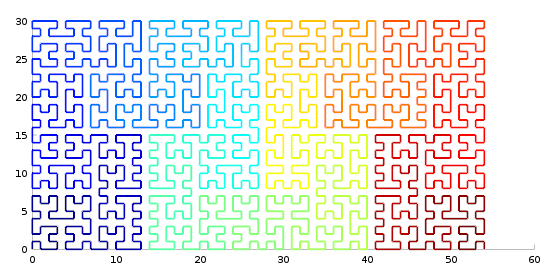
\includegraphics[width=5cm]{gilbert} }}
    \qquad
    \subfloat[\centering Four concatenated Gilbert curves\label{fig: gilbert_concat}]{{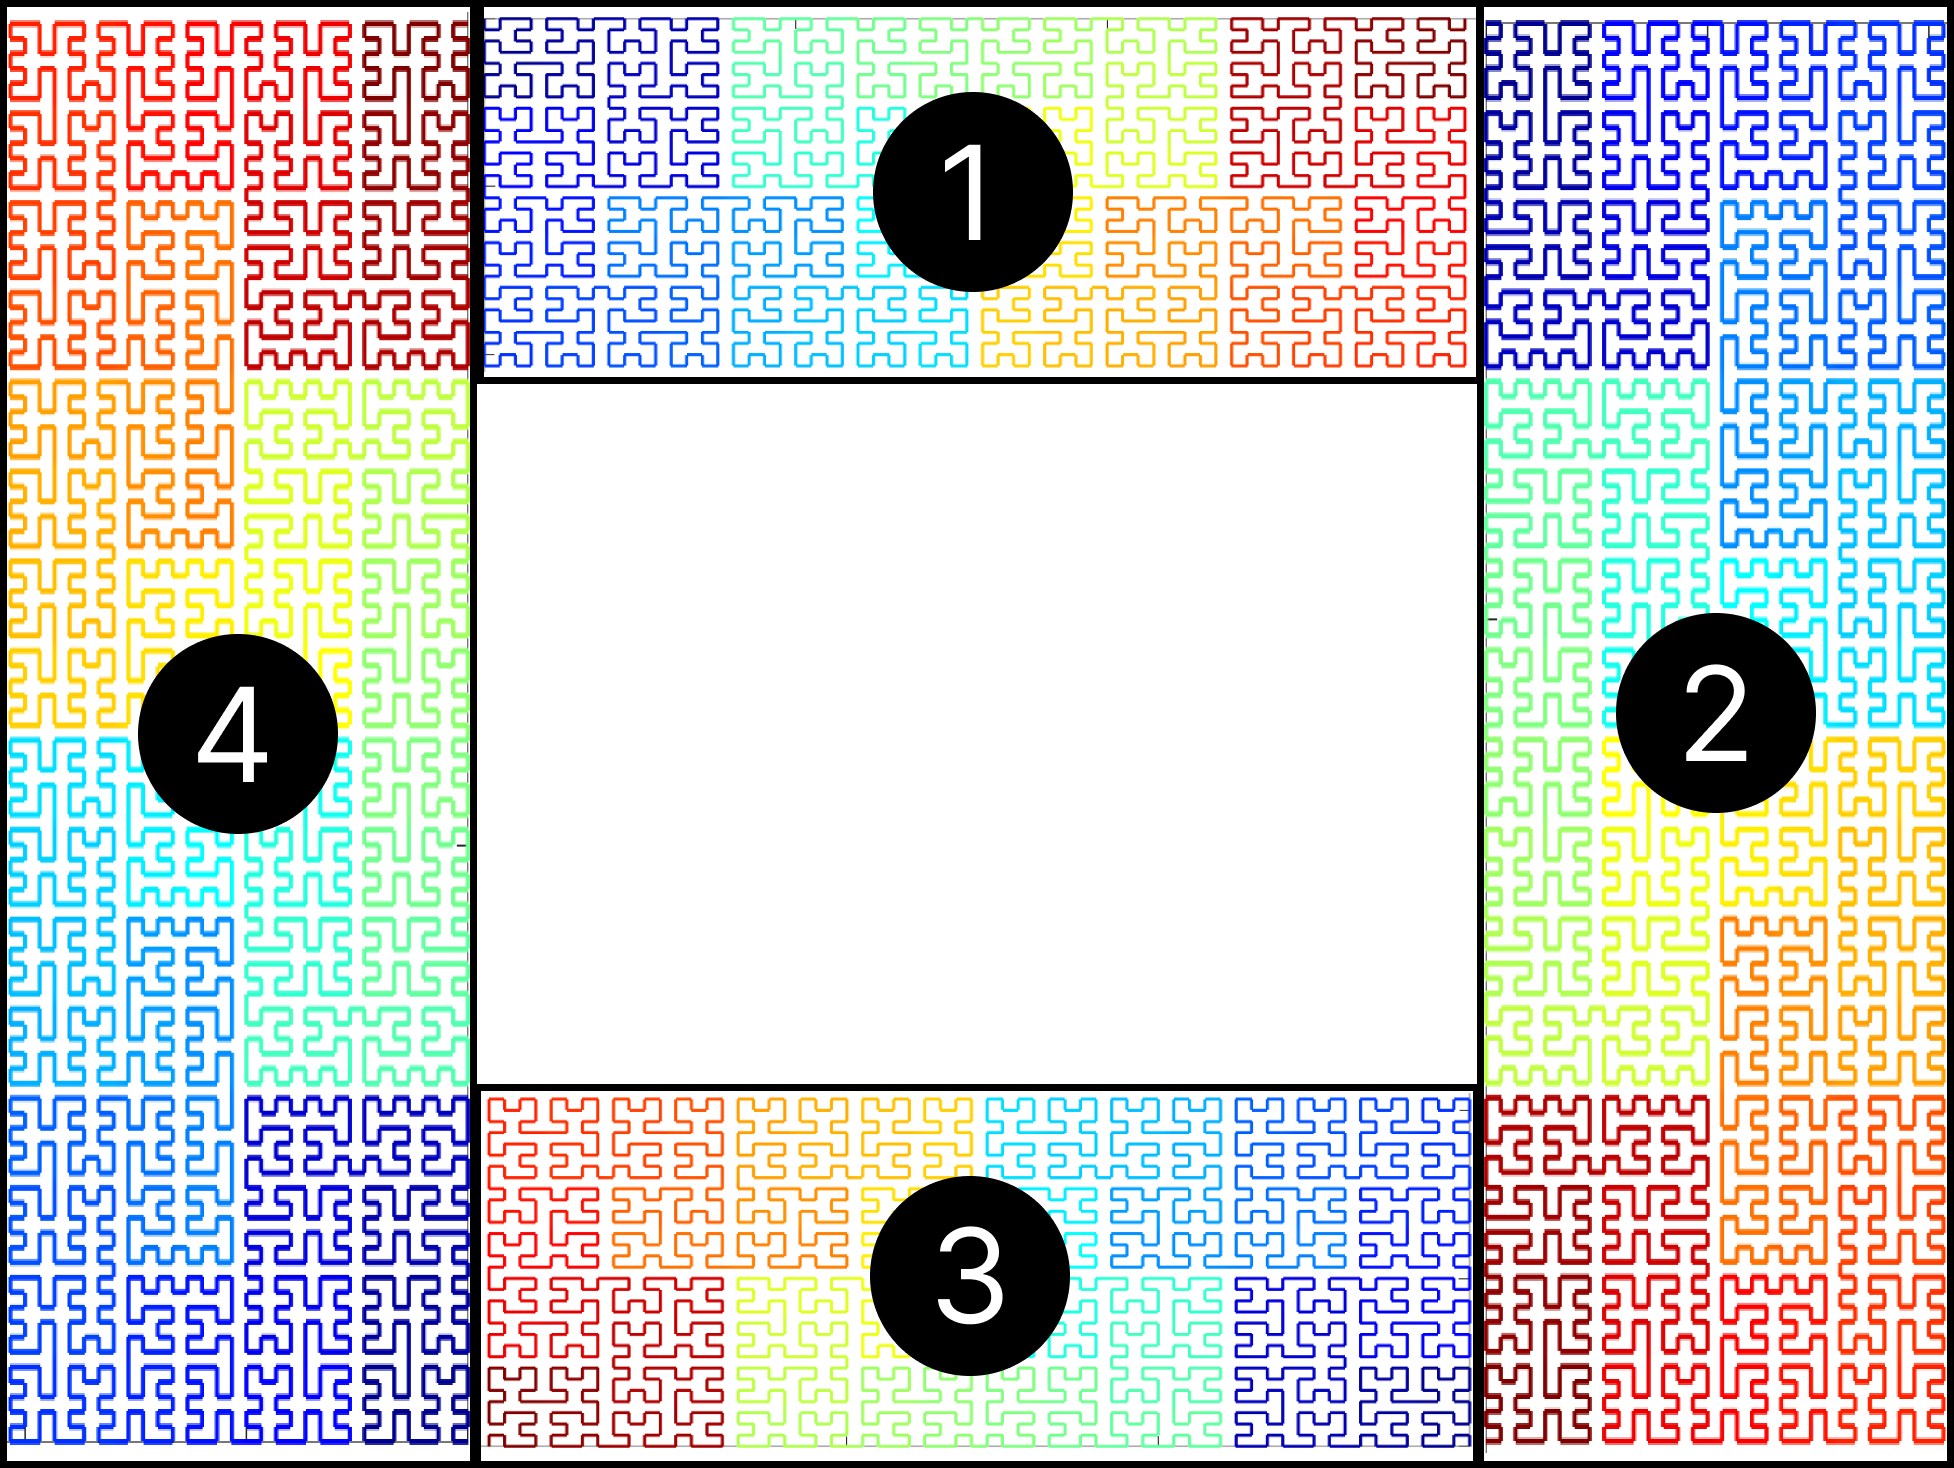
\includegraphics[width=5cm]{concatenated_gilbert} }}%
    \qquad
    \subfloat[\centering An order-4 Gosper curve\label{fig: gosper}]{{
\includegraphics[width=5cm]{gosper} }}%
    \caption{
        (a), (b): Illustration of concatenating Gilbert curves. 
        The color indicates the traverse direction of Gilbert curves: start with dark blue and end with dark red.
        (c): An example of order-4 Gosper curve used for the center area.
    }%
    \label{fig: gilbert}%
\end{figure}

\subsection{Improving the readability}
\subparagraph{Automatic Cluster Expansion}
In most cases, the default clustering result is not optimal for the user's targeted analysis tasks.
We identify two common problems in early prototyping: 
(1) clusters may be too big, weakening the semantic meaning that the clusters can convey.
(2) clusters may have only one sub-cluster, which makes the parent cluster redundant. 
Both problems can be mitigated by automatically expanding a cluster.
We employ rule-based detection to identify clusters that need to be expanded.
For a cluster $C$, we expand it if the following conditions are met:
(1) $C$ has only one sub-cluster $C_s$;
(2) $C$ has more than $n = k N$ nodes, where $k \in [0, 1]$ and $N$ is the size of the hypergraph.
Through trial and error, we find that $k=0.3$ gives the most balanced results.

\subparagraph{Spacing Strategy}
Spacing between each node is important for the readability and aesthetics of SFC layouts.
To highlight different clusters, we employ our spacing strategy on clusters instead of nodes.
Given a space-filling curve of a specific order, we first calculate the length of the curve $L$.
$L$ represents the total amount of space available for the nodes and thus,
$L - N$ represents the amount of space to be redistributed, where $N$ is the size of the hypergraph.
Our goal is to distribute the space between clusters to ensure the best readability.
In early prototyping, we found that distributing the space proportional to the cluster size gives the best readability.
Specifically, we define the space of a cluster as the blank space it has behind it on the curve, which is calculated by $(L-N)\frac{N_c}{N}$, where $N_c$ is the size of the cluster.
TODO: add a diagram here

\subparagraph{Concave hull approximation}
After applying the SFC layout, we use a concave hull algorithm~\cite{park2012concavehull} to generate an approximation polygon for each cluster.
The polygons are used to generate borders and calculate label positions for the clusters.
The concave hull algorithm is generated based on a cluster of points, in our case, the nodes in a cluster.
This means that the algorithm can be applied to any curve we used for the SFC layout.
This is a desirable property because we are using two different curves in our system, and the center area curve choice is flexible.
Using the same algorithm guarantees a unified aesthetic across curves.

The original concave hull algorithm is designed for approximating points, but we need to approximate circles.
Naively we can use the center of the circles as the points for the algorithm, but this would result in a polygon that is too small and crosses the circles on the boundary.
To address this issue we use a simple trick: we add extra points to the cluster by extrapolating the original points.
For a Gilbert curve, the curve moves perpendicularly, so the resulting polygon would have perpendicular corners. 
We can therefore add eight extra points around each original point so that the extrapolation forms a three-by-three grid.
On the boundary of the cluster, these extra points prevent the concave hull from passing across the original points.
Since the concave hull algorithm has an $O(n\log n)$ time complexity, the performance overhead introduced by the extra points is negligible.
\subparagraph{Borders} 
The borders are generated by applying a smoothing algorithm on the polygons.
For Gosper curves, we use the polygon as control points to generate a cubic basis spline as the border.
For Gilbert curves, we use a similar approach but with a cubic Bezier curve.
More specifically, for each pair of consecutive points, we use a smoothing factor to interpolate the control point.
This results in a sketchy style at the border corners.
Two examples are given in~\autoref{fig: borders}.

\begin{figure}%
    \centering
    \subfloat[\centering ]{{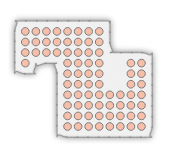
\includegraphics[width=5cm]{example_gilbert_border} }}%
    \qquad
    \subfloat[\centering ]{{
\includegraphics[width=5cm]{example_gosper_border} }}%
    \caption{(a) An example of Gilbert cluster border (b) An example of Gosper cluster borders}%
    \label{fig: borders}%
\end{figure}
\subparagraph{Labeling}
Labeling the clusters is essential for users to explore the dataset.
We use the topic assignment described in \autoref{sec: tag_assignment} to label the clusters.
When using SFC layouts, determining the label position automatically is challenging because the shape of the clusters can be irregular.
For a cluster, the label position is simply the centroid of the polygon.
When a cluster is expanded through user interaction, the sub-clusters within need to be clearly labeled as well.
Using the centroid of the sub-cluster as the label position is not a good choice because the label would cause a serious cluttering issue.
Therefore, for a sub-cluster, we first calculate the centroid of the sub-cluster, and then we extend the line from the parent cluster centroid to the sub-cluster centroid. 
Once the intersection point of the extended line and the parent border is found, we extend the line by a fixed amount to avoid any overlapping issues.
This results in a radial layout for the sub-cluster labels, as shown in~\autoref{fig: labels}.
The generalizability of the concave hull algorithm makes our labeling position calculation applicable to any curve we use for the SFC layout.
\begin{figure}%
    \centering
    \subfloat[\centering Label position of the cluster is the centroid of each cluster.]{{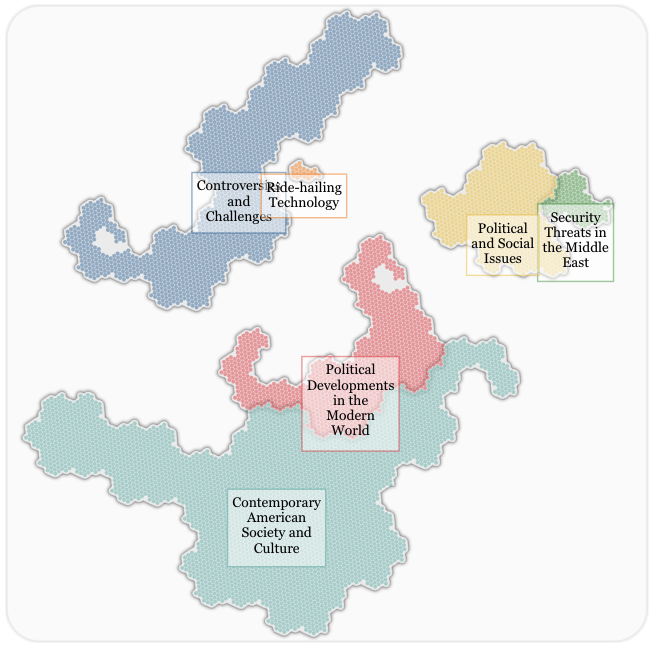
\includegraphics[width=0.5\columnwidth]{cluster_label} }}%
    \subfloat[\centering Labels of the sub-clusters of a cluster. The color indicates different sub-clusters. \label{fig: sub-cluster}]{{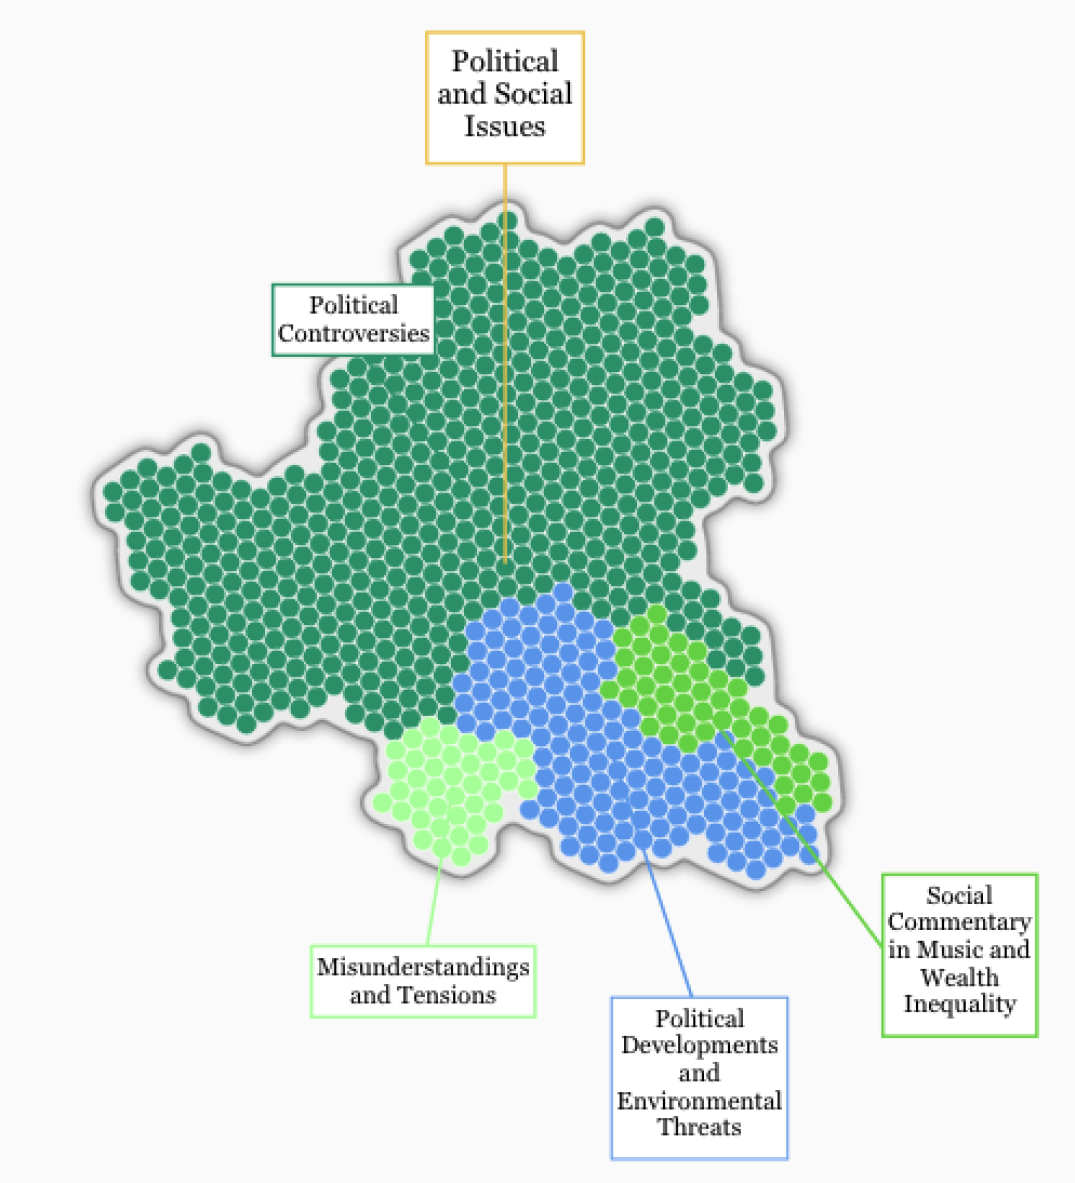
\includegraphics[width=0.5\columnwidth]{sub_cluster_label} }}%
    \qquad
    \subfloat[\centering Labels of the character cluster. The left part shows the categories of the characters as the cluster label. When documents are selected, the right part appears and shows the connected characters.\label{fig: character-cluster-label}]{{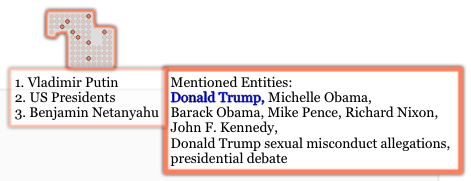
\includegraphics[width=5cm]{character_cluster_label} }}%
    \caption{(a) Labels (topics) of the document clusters (b) An example of expanded cluster labels (c) An example of character labels (categories) and highlighted characters}%
    \label{fig: labels}%
\end{figure}

% \subsection{Design Choices}
% \subparagraph{Why show all the nodes as circles}
% \subparagraph{Why hide the links}




%% if specified like this the section will be committed in review mode
\acknowledgments{
The authors wish to thank A, B, and C. This work was supported in part by
a grant from XYZ.}

%\bibliographystyle{abbrv}
\bibliographystyle{abbrv-doi}
%\bibliographystyle{abbrv-doi-narrow}
%\bibliographystyle{abbrv-doi-hyperref}
%\bibliographystyle{abbrv-doi-hyperref-narrow}

\bibliography{template}
\end{document}
